% Complete flattened LaTeX; use the accompanying figures directory.
% Canonical build: bash build_paper.sh. Sources and evidence are in the complete ZIP.
\documentclass[11pt,letterpaper]{article}
\usepackage[T1]{fontenc}
\usepackage[utf8]{inputenc}
\usepackage{mathpazo,helvet,courier,microtype}
\usepackage[margin=0.91in,headheight=16pt]{geometry}
\usepackage{amsmath,amssymb,booktabs,tabularx,array,longtable,graphicx}
\usepackage[dvipsnames]{xcolor}
\usepackage{tikz}
\usetikzlibrary{arrows.meta,positioning,calc}
\usepackage[most]{tcolorbox}
\usepackage{enumitem,fancyhdr,titlesec,caption,needspace,etoolbox,float}
\usepackage[numbers,sort&compress]{natbib}
\usepackage{hyperref}
\definecolor{Cosmic}{HTML}{32165C}
\definecolor{Aperture}{HTML}{6535B4}
\definecolor{Teal}{HTML}{087F8C}
\definecolor{Amber}{HTML}{B56A18}
\definecolor{Ink}{HTML}{222232}
\definecolor{Mist}{HTML}{F4F1F8}
\hypersetup{colorlinks=true,linkcolor=Cosmic,citecolor=Teal,urlcolor=Teal,pdftitle={AGI ALPHA: Alpha Beyond Prediction},pdfauthor={MONTREAL.AI -- Writer 11 research edition},pdfsubject={Constructing adaptable productive capabilities under deep uncertainty}}
\setlength{\parindent}{0pt}
\setlength{\parskip}{0.46em}
\linespread{1.08}
\clubpenalty=10000
\widowpenalty=10000
\displaywidowpenalty=10000
\brokenpenalty=10000
\setlist{nosep,leftmargin=1.4em,topsep=0.4em}
\titleformat{\section}{\Large\sffamily\bfseries\color{Cosmic}}{\thesection}{0.7em}{}
\titleformat{\subsection}{\large\sffamily\bfseries\color{Cosmic}}{\thesubsection}{0.7em}{}
\titleformat{\subsubsection}{\normalsize\sffamily\bfseries\color{Ink}}{\thesubsubsection}{0.7em}{}
\pretocmd{\section}{\Needspace{5\baselineskip}}{}{}
\pretocmd{\subsection}{\Needspace{4\baselineskip}}{}{}
\captionsetup{font=small,labelfont={bf,sf},skip=7pt}
\newtcolorbox{finding}[1][]{colback=Mist,colframe=Cosmic,boxrule=0pt,leftrule=2.2pt,arc=0pt,left=12pt,right=12pt,top=9pt,bottom=9pt,#1}
\newcommand{\ap}{\textsc{Aperture}}
\newcommand{\code}[1]{\texttt{\small #1}}
\newcommand{\unk}{\textit{unknown}}
\newcommand{\yes}{\textsf{executed}}
\pagestyle{fancy}
\fancyhf{}
\fancyhead[L]{\sffamily\small\color{Cosmic}AGI ALPHA \; / \; ALPHA BEYOND PREDICTION}
\fancyhead[R]{\sffamily\small MONTREAL.AI}
\fancyfoot[L]{\sffamily\scriptsize Research edition \;\textbullet\; bounded digital evidence}
\fancyfoot[R]{\sffamily\small\thepage}
\renewcommand{\headrulewidth}{0.3pt}
\newcommand{\artifactpath}[1]{\path{#1}}
\begin{document}
\color{Ink}
\hypersetup{pageanchor=false}
\begin{titlepage}
\thispagestyle{empty}
\begin{tikzpicture}[remember picture,overlay]
\fill[Cosmic] (current page.north west) rectangle ([yshift=-2.2in]current page.north east);
\foreach \x/\y/\r in {1.3/1.2/.02,5.8/.5/.018,6.7/1.4/.025,3.3/.7/.013,7.6/.4/.02,2.3/1.8/.015,4.8/1.7/.02}
{\fill[white,opacity=.65] ([xshift=\x in,yshift=-\y in]current page.north west) circle (\r in);}
\draw[white,opacity=.4,line width=.5pt] ([xshift=5.5in,yshift=-1.6in]current page.north west) arc (190:345:1.25in and .45in);
\end{tikzpicture}
\vspace*{.22in}
{\sffamily\color{white}\large MONTREAL.AI \hfill RESEARCH / 11}\par
\vspace{.37in}
{\sffamily\color{white}\fontsize{18}{22}\selectfont AGI ALPHA}\par
\vspace{1.02in}
{\sffamily\bfseries\color{Cosmic}\fontsize{38}{41}\selectfont ALPHA BEYOND\\PREDICTION}\par
\vspace{.28in}
{\sffamily\fontsize{17}{23}\selectfont Constructing Adaptable Productive Capabilities\\Under Deep Uncertainty}\par
\vspace{.42in}
{\color{Teal}\rule{.9in}{2pt}}\par
\vspace{.18in}
{\fontsize{20}{27}\selectfont Build the instrument.\\Let the question change.}\par
\vspace{.3in}
\begin{finding}
A complete, executable investigation of a small scientific capability that can change its measurement program as demand changes. Its claims are bounded by frozen experiments, equally enabled conventional methods, and failures that remain visible.
\end{finding}
\vfill
{\sffamily\bfseries MONTREAL.AI}\par
{\small Writer \#11 research edition \;\textbullet\; 23 October 2026 (Toronto)}\par
{\small AI-assisted research, implementation, evaluation and publication.\\Digital laboratory; no wallet, paid API, financial transaction or physical instrument required.}\par
\vspace{.15in}
{\footnotesize Source and evidence accompany this manuscript. Neither a successful fit nor a bloom is proof of profit.}
\end{titlepage}
\hypersetup{pageanchor=true}

\section*{Abstract}
What useful means of production can be built before we know which task will matter? We study this question through \ap{}, a bounded scientific program that constructs measurement operators from a finite expression language, then selects observations, fits conventional models and adapts to permitted evidence. The artifact supports spectral characterization, causal system identification and a previously hidden spatial count-imaging family. A public NIST pilot first establishes that ordinary known-model fitting is already cheap. We then freeze the scientific implementation and protocol before revealing the third family, and evaluate eight methods on 96 synthetic missions, producing 768 records. The proposed implementation and an equally enabled conventional modular construction control both qualify in 54/96 missions, choose the same actions, and consume the same acquisition and verification units. The held-out family qualifies in only 6/32 cases. A model-based residual verifier accepts all 94 completed missions, including 40 scientifically unacceptable estimates; two further missions abstain on authority. A conventional Gaussian likelihood substitute matches qualification on every case, while uniform design loses four qualifications. Finite demand-sequence replays show conditions in which switching consumes capacity and waiting avoids unrecovered losses. The contribution is an inspectable construction and evaluation package, with an honest negative method comparison and a concrete warning about shared-model verification. It is not a new theory of optionality, evidence of physical deployment, or a claim of economic returns. Human engineering and monetary costs remain unmeasured. Source, frozen hashes, all outcomes, a local three-minute demonstration and restoration tests accompany the paper.

\par\vspace{.4em}
{\small\sffamily\textbf{Keywords:} adaptable capability; deep uncertainty; experimental design; scientific software; modularity; bounded authority; reproducible negative results.}

\begin{finding}
\textbf{Reading this paper.} A laboratory can be valuable because it can answer a question that was not its original assignment. That does not mean its architecture beats a competent conventional laboratory. We separate these claims and test both. The complete source package contains the frozen program, every case, recorded failures, a local interactive demonstration, and the commands used to rebuild this paper.
\end{finding}

\section{An instrument for the question that changes}

Suppose a small scientific team first needs to measure the composition of a material. Later, the useful assignment is to identify how a dynamical system responds to an input. Later still, it needs to configure an instrument for another measurement process. Predicting the third assignment correctly would help. Building an instrument that can be reconfigured may also help. The engineering question is whether the second approach actually changes what the team can do, at a cost it can justify.

The motivating AGI question asks which sector will transform first. Here we replace a sector forecast with a construction problem: \emph{what productive capability can be built before demand is known, and what remains possible when demand changes?} The object of study is executable scientific machinery: a representation of measurements, an inference engine, a bounded policy for selecting observations, and an evidence record that survives changes of task. It is not a basket of securities or an allocation across unrelated activities.

Consider two distinct reasons for flexibility to look valuable. A fixed spectral tool cannot execute a new count-measurement mission; a general builder can construct the necessary operator. This demonstrates an expanded attainable task set relative to the fixed tool. But if a conventional modular builder can construct exactly the same operator with the same information and methods, the new architecture has not established a method-specific advantage. Both comparisons matter. Confusing them would turn a sensible engineering choice into a misleading claim of superiority.

\ap{} is the concrete artifact investigated here. A mission describes mathematical response functions, candidate measurements, an observation law, costs and explicit local permissions. The program constructs its observation operator, fits a conventional model, selects measurements, reacts to newly revealed health evidence, and exports World, Policy, Proof and Authority objects. An initial spectral point experiment can become a causal experiment with a forcing history, or a different aggregate measurement process. Changes outside the installed finite language are refused rather than invented after the test is seen.

The study makes three contributions of limited, inspectable scope. First, it provides a complete small implementation in which a changed measurement representation, likelihood and admissible observation set can be traced to actual numerical work. Second, it supplies a frozen, role-separated evaluation protocol with an equally enabled conventional builder, an explicit capability ablation, a numerical representation replacement, a likelihood substitute, a waiting policy and a privileged scenario specialist. Third, it reports when the proposed machinery works, ties, fails, or becomes unnecessary. These are contributions of engineering synthesis and evaluation, not a new theory of optionality or a discovery algorithm for arbitrary scientific tasks.

\subsection{What ``alpha'' means in this study}

For a stated task set and comparator, alpha is a measured difference in scientific coverage, task error or resource consumption at a stated quality level. A positive difference is not presumed. The baseline is permitted to build reusable capabilities. Human engineering effort and economic prices are not available, so neither equal human budgets nor positive net economic value can be inferred from a numerical tie or a difference in computer time.

The project source's \$15 quadrillion phrase is treated only as motivating language. Its currency, horizon and accounting perimeter are not instantiated in this paper. It is not a forecast, available market, valuation, wealth estimate or input to any result. Removing that magnitude leaves every experiment and conclusion unchanged. Section~\ref{sec:foundations} records the source caveat and the distinction between a scientific output, a contract state and a realized receipt.

\section{Known foundations and the narrower contribution}

Robust optimization has long made uncertainty sets and the cost of protection explicit. Bertsimas and Sim study the price of robustness; Ben-Tal and colleagues distinguish decisions made before uncertainty resolves from adjustable decisions made afterward \citep{bertsimas2004price,bental2004adjustable}. Deep-uncertainty methods examine policies across alternative futures rather than treating one unsupported probability model as known. Robust decision making and dynamic adaptive policy pathways provide direct antecedents for contingent action and monitored change \citep{lempert2003shaping,haasnoot2013pathways}. Our finite stress suite does not solve a general robust optimization problem. Its weights are diagnostic choices, not estimated probabilities of future demand.

Waiting under irreversibility is also established. McDonald and Siegel analyze the value of delaying an irreversible investment under specified stochastic assumptions \citep{mcdonald1986waiting}. Here waiting is an executable refusal to consume a limited experimental budget. Our replay uses abstract reward sensitivity and explicitly assumed switching tariffs. It is not an empirical estimate of a real option price.

Reconfigurable manufacturing treats structure and functionality as engineering choices that should change with production requirements \citep{koren1999reconfigurable}. Parnas's information-hiding criterion and Baldwin--Clark's modular design analysis explain why interfaces may localize change, while also introducing architectural costs \citep{parnas1972modules,baldwin2002option}. The direct analogue is a measurement interface that separates a public scientific model from a shared solver and an authority record. Calling that separation transformational does not make modularity new.

Program synthesis and scientific model compilation are similarly important precedents. Sketching searches within a supplied partial program and specification; ModelingToolkit composes graph transformations to generate numerical implementations \citep{solarlezama2008sketching,ma2021modelingtoolkit}. \ap{} does not learn its language or synthesize arbitrary programs. It constructs a finite numerical operator from supplied expressions and applies installed procedures. Sparse identification of nonlinear dynamics illustrates a much stronger data-driven model-discovery objective, which this study does not claim to reproduce \citep{brunton2016sindy}.

The numerical ingredients are conventional. Separable nonlinear least squares, sensor-selection methods and Bayesian experimental design provide relevant alternatives and a warning against weak baselines \citep{golub1973separable,joshi2009sensors,foster2019design}. We retain standard least-squares and Poisson optimization rather than replacing them merely to create novelty. The primary modular comparator receives the same primitives and decision rule; a separate numerical test suite checks our fits against independently formulated conventional objectives.

\begin{table}[htbp]
\centering\small
\begin{tabularx}{\linewidth}{@{}p{.23\linewidth}XX@{}}
\toprule
\textbf{Status} & \textbf{What belongs here} & \textbf{What is not established}\\
\midrule
Known foundations & Robust/adaptive decisions, modularity, option value, experimental design, model compilation & Priority over these fields\\
Engineering synthesis & One bounded measurement program, evidence ledger, current-authority restoration and a reproducible demo & Autonomous invention of its primitives\\
Proposed contribution & Auditable structural adaptation and a matched construction comparison across different scientific missions & General transfer beyond the finite language\\
Observed result & Complete fixed-case numerical outcomes, costs, refusals and false acceptances & Physical validity or commercial adoption\\
Open hypothesis & Whether additional architecture reduces future engineering or verification effort & A positive total-cost or market-value advantage\\
\bottomrule
\end{tabularx}
\caption{Intellectual positioning. The implementation is useful even when its distinctive architecture supplies no numerical advantage over an equally enabled conventional builder.}
\end{table}

\section{Problem definition: construct first, commit later}

\subsection{The object being constructed}

A public mission is a tuple
\begin{equation}
M=(\Phi,\mathcal A,\ell,\eta,b,V_q,\tau),
\end{equation}
where $\Phi=(\phi_1,\ldots,\phi_p)$ is a finite response basis, $\mathcal A$ is a set of candidate measurement actions, $\ell$ is the declared likelihood, $\eta$ contains known noise or exposure parameters and priors, $b$ is the acquisition-unit budget, $V_q$ is the reserved verification procedure and $\tau$ is the scientific quality threshold. A separate authority declaration binds the immutable mission digest, scope, resource ceiling and validity interval. The declaration is a local research fixture; it is not a credential or a grant of external access.

Each action $a$ contains points $x_{aj}$, weights $w_{aj}$, cost $c_a$, and an instrument-group identity. Construction produces the row
\begin{equation}
A_{ak}=\sum_j w_{aj}\phi_k(x_{aj}).\label{eq:operator}
\end{equation}
Weights encode the physical measure of the declared digital model. They are not silently normalized: a sum, average and path integral need not represent the same experiment. A point measurement is a special case of Equation~\eqref{eq:operator}; a temporal response may contain a complete forcing history inside $\phi_k$. This changes actual constructed numerical work, although it does not escape the common finite-dimensional inverse-problem structure.

For Gaussian missions,
\begin{equation}
y_a=A_a\theta+Z_a\gamma+\epsilon_a,
\qquad \epsilon_a\sim\mathcal N(0,\sigma^2),\label{eq:gaussian}
\end{equation}
where $Z\gamma$ is the explicitly declared nuisance model. For count missions,
\begin{equation}
y_a\sim\operatorname{Poisson}\!\left[e\left(\beta+A_a\theta\right)\right],
\qquad \theta\geq0,\quad\beta>0.\label{eq:poisson}
\end{equation}
Shared calibration faults deliberately violate the fitted observation model unless newly available evidence permits a conservative response. They are retained as failures of the assumptions, not relabeled as successful robustness.

\subsection{Information, policies and purpose}

At step $t$, the policy has the current mission, observations it actually requested, currently valid authority and health evidence revealed by that time. It does not receive hidden coefficients, evaluation labels, future demand or the future health-event schedule. A simulator callback returns one requested observation. Noise streams are keyed by case, action and repetition, so an alternative action order does not create a favorable private noise realization.

The hidden scientific evaluator uses a separate noiseless validation operator $H$ and computes
\begin{equation}
E(M,\widehat\theta)=
\frac{\sqrt{\operatorname{mean}\left[(H\widehat\theta-H\theta)^2\right]}}
{\max\left(\sqrt{\operatorname{mean}[(H\theta)^2]},10^{-8}\right)}.
\end{equation}
Scientific feasibility is $E\leq0.12$. Qualified output additionally requires the predeclared residual verification check. This purpose bridge keeps an internally confident but scientifically wrong model from becoming a success merely because its own judge agrees with it.

For a finite set of cases $\mathcal S$, define $Q_s(\pi)$ as qualified-output indicator and $\mathbf C_s(\pi)$ as the recorded cost vector. The primary paired comparison is
\begin{equation}
\Delta Q_s=Q_s(\pi_{\rm Aperture})-Q_s(\pi_{\rm modular}),\qquad
\Delta\mathbf C_s=\mathbf C_s(\pi_{\rm Aperture})-\mathbf C_s(\pi_{\rm modular}).
\end{equation}
No distribution over real future demand is assumed. A weighted sum $\sum_s p_s\Delta Q_s$ is meaningful only as a chosen mixture of these observed cases. It cannot guarantee performance for an unrepresented task family.

\subsection{Authority is outside the optimization objective}

Scientific desirability does not create permission. A missing grant, expired assignment or incompatible mission hash stops execution. Waiting is allowed for at most three ticks when the grant is explicitly future-dated. Materially new work gets a new immutable mission and a fresh bounded declaration; the old plan remains inspectable. A health warning may only narrow the already authorized action set. It does not authorize a new instrument, a different scientific objective or a numerical correction derived from hidden truth.

Restoration requires both an intact saved bundle and a separately supplied current authority context. The context must not be recovered from the untrusted imported bundle. Ordinary hashes detect byte changes relative to known bytes; they do not authenticate an actor or certify scientific truth. The tests therefore attack edited expiry, recomputed hashes, changed missions and incompatible program identity, while keeping the current grant outside the imported object.

\section{How the adaptable capability is built}

\subsection{A small language, a real transformation}

The pre-reveal library includes constants, coordinates, addition, multiplication, exponentials, sine, cosine, Gaussian responses and causal exponential responses to an explicit impulse history. The grammar is bounded to eight latent coefficients, 160 candidate actions and 256 quadrature points per action. Recursion depth, arity, finite values, action costs and likelihood constraints are validated. Unsupported expressions fail explicitly. Public inputs contain no executable source string and are never passed to an unrestricted evaluator.

Before demand is revealed, the builder implements aggregation, inference, design, accounting, quarantine and restoration. After reveal, a public mission supplies an arrangement of those primitives. This constructs a concrete operator and execution plan. The distinction is important: the prebuilt machinery is reusable, but the final measurement program does not exist until the mission is composed. An unsupported law or an unknown primitive still requires replacement or a new development episode.

Temporal system identification is not renamed spectroscopy. Its columns are causal responses to a known forcing history and its task is to identify dynamic response coefficients. Spectral characterization uses localized wavelength responses and an unknown baseline. The held-out task changes the observation geometry and law. Nevertheless, all are small inverse problems. They do not establish transfer to arbitrary enterprise work, autonomous scientific discovery or unknown physical laws.

\subsection{Conventional inference and bounded design}

For Gaussian data, the implementation solves a diagonal weighted ridge/MAP problem jointly over target and nuisance coefficients. An independent test constructs the augmented least-squares system and compares its solution and covariance numerically. This is not a claim of general dense-covariance GLS.

For Poisson observations, standard L-BFGS-B minimizes the negative log likelihood plus a quadratic prior penalty under nonnegative coefficient bounds. Its inverse expected Fisher information plus prior precision supplies an approximate design covariance. Independent tests compare the objective and optimum with a separately formulated constrained optimizer. Negative, fractional and nonfinite counts are not admitted as valid counts; their acquisition costs remain in the ledger.

Given current covariance $C_t$ and conditional noise scale $v_a$, let $d_a=[A_a,Z_a]$ for a joint Gaussian target/nuisance fit and $d_a=A_a$ for the count model. The acquisition rule is the familiar greedy information score
\begin{equation}
a_t\in\arg\max_{a\in\mathcal A_t,\;c_a\leq b_t}
\frac{\log\!\left(1+d_aC_td_a^\top/v_a\right)}{c_a}.
\end{equation}
Canonical tie-breaking makes numerical representations directly comparable. Three repeats per action and 48 selection iterations bound execution. Every row actually scored is counted, including rows later masked as infeasible. Feasible-candidate counts are recorded separately. Model construction and numerical candidate scoring are computations; they are not detector acquisitions.

\subsection{Adaptation when evidence changes}

A delayed group-level calibration suspicion reveals no exact correction factor. The fixed response removes the affected actions, excludes their earlier observations from fitting, refits on surviving data and preserves the sunk acquisition costs. The plan hash does not change: using fewer preauthorized actions is allowed, while expanding the mission is not. Quarantine is an actual change in the data set and execution structure, not a caption added after the fact.

Four reserved verification actions follow fitting. Their normalized residual statistic includes assumed measurement noise and fitted parameter uncertainty; the predeclared acceptance threshold is four. Verification observations do not retrain the estimate. If a new health warning arrives during verification, earlier verification scores are discarded. The budget is not silently enlarged to obtain another four observations; insufficient fresh evidence means no acceptance.

This checker is deliberately treated as fallible. Common calibration errors can preserve internal residual agreement while moving the answer away from the hidden scientific target. Reporting that disagreement is part of the result. A digest, a clean log or multiple agreeing model-based checks cannot substitute for an independent outcome anchor.

\section{Development, registration and confirmation}

\subsection{A public-data pilot that removed a false bottleneck}

NIST Gauss1 is a generated, lower-difficulty nonlinear-regression reference with 250 observations, two supplied starting points and certified numerical values \citep{nist1996gauss1}. We used the ordinary SciPy least-squares solver. The residual sums of squares from both starts were approximately $1315.82224320338$, differing from the rounded certified value by $2.57\times10^{-12}$ relatively. Instrumented fits took approximately 3--4 milliseconds, with 54 and 64 actual residual calls including numerical-Jacobian evaluations. These observations establish that known-model fitting was already cheap in this pilot. They provide no evidence for physical characterization or a new optimization algorithm.

The measured script body, including numerical imports, reading, fitting and derived CSV writing, took about 1.004 seconds wall time and 2.142 seconds CPU time in its recorded environment; interpreter startup and final JSON serialization were excluded. Full machine time differs from solver time. Attributable human effort and model-provider computation were not measured.

StRD is NIST SRD 140. Its dataset-specific instructions invite downloading, analyzing and comparing reference data, but we did not establish blanket redistribution rights for the raw observations \citep{nistlicense}. The publication therefore supplies a retrieval URL, exact input hash, analysis script, aggregate/parameter results and fitted-curve outputs. It excludes the raw input and residual columns that could reconstruct it. The reader can regenerate those locally after retrieving the source.

\subsection{What was frozen and what was hidden}

The initial registration and pilot were saved first. A separate evaluator then sealed a generator without materializing or scoring any hidden cases. A generic interface review disclosed schema compatibility issues, not the exact family or parameters. The full scientific source, protocol, analysis and 22 independent checks were frozen before reveal. The frozen checkpoint was saved, reopened and verified; the coordination thread records its hash before reveal authorization.

The final source/protocol freeze is
\begin{center}\footnotesize\ttfamily
147678382894e349fd53236e68447cb640110e25aa401ae5c7f19d0be6528076
\end{center}
The complete checkpoint hash and all 39 frozen file identities are in the package. The hidden generator's original archive is preserved unchanged. The scientific source is not tuned after reveal. Any wrapper reconciliation or later defect must be reported with its own chronology and cannot silently convert the original study into a new confirmatory claim.

This is same-session procedural role separation. The agents share a filesystem; there is no cryptographic barrier or independent institution. The protocol makes the chronology inspectable and the policy's information boundary executable. It cannot prove that an untrusted investigator had no possible access. The generator becomes public after the study so readers can reproduce it.

\subsection{Sampling, conditions and costs}

There are 64 fresh cases in the two known families: seeds 101--108 crossed with four conditions for each family. A further 32 cases come from the previously hidden family, eight per condition. The conditions cover nominal operation, correlated calibration failure, capacity loss and delayed authority/evidence. Eight methods yield 768 primary records. No failed case is removed from the denominator.

The primary budget is 24 fitting acquisition \emph{units}, with published reductions in capacity cases, followed by four validation actions whose actual costs are recorded separately. A cost-one action and a multi-unit aggregate action are different resource commitments. The paper does not describe every mission as having 24 plus four acquisitions. The general authority ceiling conservatively reserves the fitting budget plus four maximum-cost validation actions.

The cost vector retains construction node evaluations and rows, acquisitions and resource units, verification work, all numerical row scores, optimizer calls, recovery, waits, wall time and CPU time. Physical instrument time, energy, monetary tariffs, long-lived maintenance, human engineering, reviewer effort and model-provider resources are unknown. The resulting ledger is detailed but not complete economic accounting. Unknown entries are not zero.

\section{Comparators that can build the same thing}

The \textbf{conventional modular builder} is the primary comparator. It shares the expression interpreter and constructs the same response functions using ordinary NumPy operations. It receives the same observation callback, inference routine, design rule, authority and health evidence. Its row aggregation uses weighted summation where \ap{} uses weighted matrix multiplication. It can create new measurement operators and perform the same structural adaptation. It is a same-powers conventional construction/equivalence control, not an independently engineered expert system or a recruited human expert. Shared mathematics intentionally makes a numerical tie possible and removes differences in solver quality as a source of apparent novelty.

The \textbf{flat numerical replacement} first constructs and charges for the operator, then serializes its arrays and contract and executes without the symbolic representation. The loader binds every field, including costs, availability and verification budget, to the original plan. This is a postconstruction representation intervention; it does not remove the cost of constructing the matrix. Equality shows that the symbolic structure is not necessary for the resulting numerical answer, not that all representations are equally maintainable.

The \textbf{uniform strategy} retains inference and authority while selecting a fixed spread of feasible measurements. The \textbf{Gaussian surrogate} replaces the exact count likelihood with a conventional prior-weighted Gaussian approximation; Gaussian missions are unchanged. The \textbf{frozen spectral specialist} lacks the constructed capability for a different family and abstains. It is a restricted capability ablation, never the main evidence for superiority. The \textbf{wait policy} consumes no scientific construction or acquisition resources and produces no output.

Finally, the \textbf{hindsight scenario specialist} knows the true calibration operator and failed-action identities and uses true latent coefficients in the count-design weights. It retains the same realized measurement noise and validity timing. This is a privileged, greedy scenario-informed upper reference, not an implementable ex-ante policy or a proved global performance bound. It may lose on an individual noisy case. Its privilege is recorded in every result.

The methods have matched mathematical access and operational budgets. They do not establish equal counterfactual human engineering effort. Their shared implementation also correlates defects. Independent numerical and interface tests reduce that risk, while the conventional replacement prevents a restricted static menu from serving as a straw comparator.

\section{Results: an executable capability, without a comparative premium}\label{sec:results}

\subsection{Construction and scientific delivery are different outcomes}

The frozen program accommodates three measurement structures: localized spectral responses, causal responses to a forcing history, and the revealed coded-aperture emission-imaging family. The last uses weighted spatial masks and a Poisson observation law. Its public mission is composed inside the installed language; no new primitive or solver is added after reveal. Figure~\ref{fig:branches} separates the conceptual construction boundary from one actually recorded synthetic replay. Neither establishes that a customer changed assignments or that future demand was anticipated.

\begin{figure}[htbp]
\centering
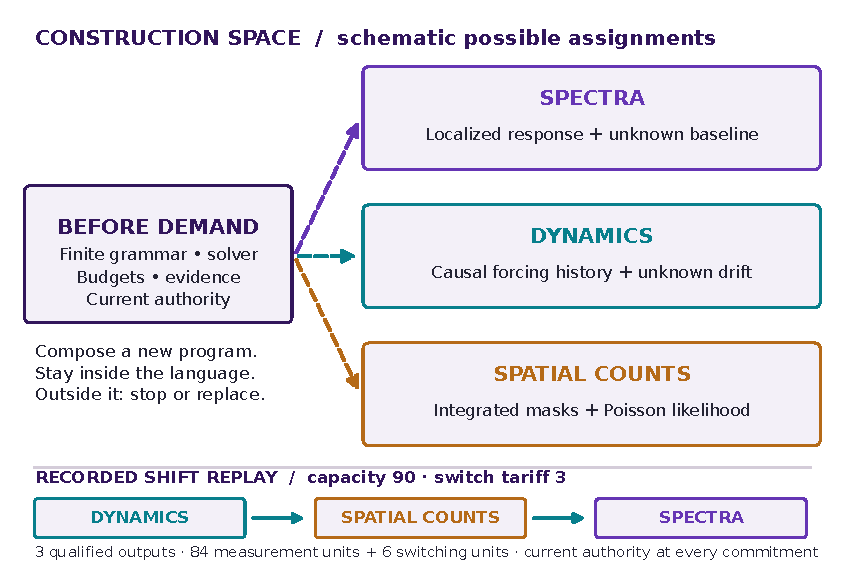
\includegraphics[width=\linewidth]{figures/capability-branches.pdf}
\caption{\textbf{Illustration above; recorded replay below.} The branches show the construction space: shared machinery precedes demand, and a mission supplies response functions and measurements. The lower path is the actual synthetic shift replay, dynamics $\to$ spatial counts $\to$ spectra, at capacity 90 and switch tariff 3: three qualified outputs consume 84 measurement units plus six switch units. This observed digital path is not a physical deployment or an anticipated customer future.}
\label{fig:branches}
\end{figure}

Executable construction does not assure a useful answer. \ap{} qualifies 54 of 96 missions, or 56.25\%, under the predeclared quality and verification requirements. Each known family qualifies 24/32; the held-out family qualifies only 6/32. Thus the study demonstrates bounded structural adaptation and substantial scientific failure together. All 96 missions remain in coverage denominators, including two authority refusals.

\subsection{The primary paired result is a tie}

The conventional modular control also qualifies 54/96, with no qualification disagreement in any paired case. Acquisition and verification action traces, including repetition and timing indices, agree throughout. Maximum absolute NRMSE difference is $1.046\times10^{-6}$: the answers are numerically close, not universally bitwise identical. Fitting and verification units, constructed rows and scored rows agree. Optimizer-call counts and measured execution times can differ.

This comparison deliberately gives conventional construction the same powers. More narrowly, both paths share the expression interpreter and all inference, design, health and authority code. Their aggregation differs between weighted matrix multiplication and an explicit weighted NumPy sum. It is therefore a conventional construction/equivalence control, not an independently engineered expert system. Its mathematical tie is expected. It rules out attributing the available task set to a numerical advantage of the new architecture, while leaving maintainability and development effort unmeasured.

\begin{table}[htbp]
\centering\small
\begin{tabularx}{\linewidth}{@{}Xrrrrrr@{}}
\toprule
\textbf{Method} & \shortstack{\textbf{Qual.}} & \shortstack{\textbf{Check}\\\textbf{passes}} & \shortstack{\textbf{False}\\\textbf{accepts}} & \shortstack{\textbf{Abstain}} & \shortstack{\textbf{Fit}\\\textbf{units}} & \shortstack{\textbf{Verify}\\\textbf{units}}\\
\midrule
\ap{} & 54 & 94 & 40 & 2 & 2,064 & 376\\
Modular control & 54 & 94 & 40 & 2 & 2,064 & 376\\
Flat replacement & 54 & 94 & 40 & 2 & 2,064 & 376\\
Uniform selection & 50 & 94 & 44 & 2 & 2,064 & 376\\
Gaussian surrogate & 54 & 94 & 40 & 2 & 2,064 & 376\\
Frozen spectral & 24 & 32 & 8 & 64 & 672 & 128\\
Wait & 0 & 0 & 0 & 96 & 0 & 0\\
Hindsight specialist & 75 & 94 & 19 & 2 & 2,064 & 376\\
\bottomrule
\end{tabularx}
\caption{\textbf{Measured confirmation outcomes.} Every row covers the same 96 missions. Qualification requires independent scientific quality and residual verification. False acceptance means verification passes but scientific quality fails. Resource units are synthetic acquisition costs; they include unsuccessful missions. The hindsight row has information unavailable to implementable policies.}
\label{tab:primary-results}
\end{table}

The flat numerical replacement likewise changes neither qualification nor selected actions. Because it pays to construct the operator before lowering and reloading its arrays, this intervention tests the necessity of symbolic structure \emph{after construction}. It does not establish that constructing a representation is free. Across every observed family/stress stratum, Aperture-minus-modular coverage and acquisition differences are zero. Any convex reweighting of these particular strata preserves those zero differences; nothing follows for an unrepresented future.

\subsection{A verifier that accepts scientifically wrong answers}

The residual check accepts all 94 completed \ap{} estimates, including 40 that fail independent scientific quality. The false-acceptance fraction is therefore 40/94, or 42.6\%, among accepted outputs; 40/96, or 41.7\%, is the distinct fraction among all missions. The remaining two missions abstain on authority timing. Verification rejects none of the completed estimates in this suite.

Figure~\ref{fig:coverage} separates the failure patterns. In each known family, all eight nominal, capacity and delayed-authority cases qualify, but all eight calibration cases fail scientific quality while passing verification. Held-out imaging qualifies 3/8 normal cases, 0/8 calibration cases, 1/8 unavailable-group cases and 2/8 delayed-authority cases. Its 30 accepted estimates contain 24 false acceptances. The two authority refusals occur in the delayed condition.

\begin{figure}[htbp]
\centering
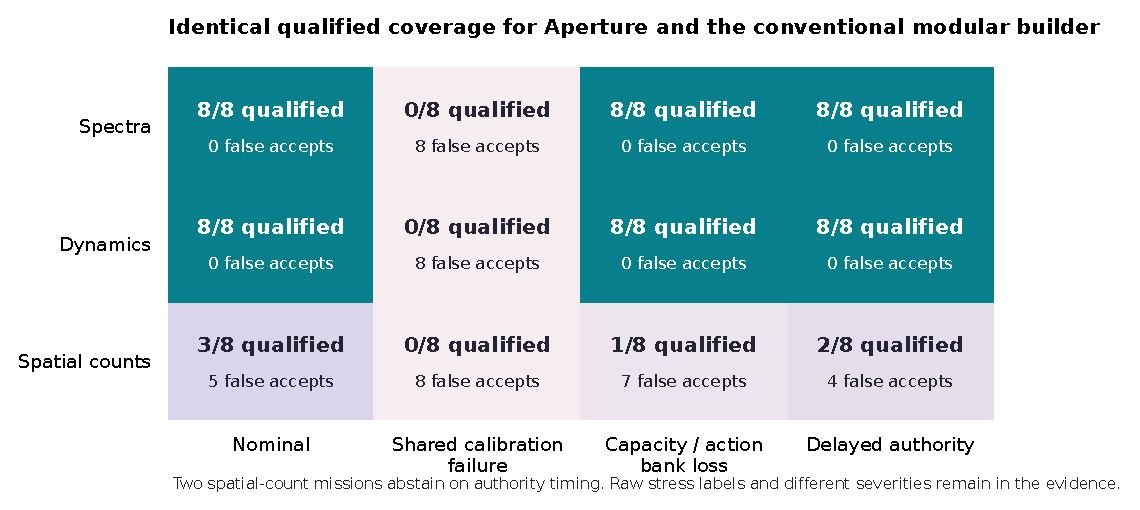
\includegraphics[width=\linewidth]{figures/coverage-and-false-acceptance.pdf}
\caption{\textbf{Measured coverage and false acceptance.} Each cell contains eight cases. Aperture and modular have identical qualification and false-acceptance counts. Column labels group related stress categories; action-bank loss and a reduced fitting budget are not identical interventions. Original labels and severities remain in the records.}
\label{fig:coverage}
\end{figure}

An elementary identifiability example explains why internal agreement can fail. In a noiseless submodel with unknown common gain $g>0$,
\begin{equation}
y=gA\theta=A\theta',\qquad \theta'=g\theta.
\end{equation}
Without an independent gain anchor, a model fitting $\theta'$ can agree with further measurements from the same instrument. For a nonzero independent linear target $H\theta$, its normalized prediction error is
\begin{equation}
\frac{\|H\theta'-H\theta\|_2}{\|H\theta\|_2}=|g-1|.
\end{equation}
This is an explanatory submodel, not a new theorem or an exact formula for every noisy, regularized case. It clarifies the known-family errors near the imposed 32\% gain shift. Delayed group suspicion permits quarantine, but does not disclose a calibration factor or create an independent reference.

Figure~\ref{fig:errors} retains individual errors. For Aperture's 94 finite estimates, median NRMSE is 0.0362, the empirical 90th percentile is 0.3328, and the maximum is 0.5548. These are conditional finite-suite summaries, not confidence bounds over future assignments. Restricted-specialist errors exist for only 32 missions; its lower pooled median cannot establish superiority on the common 96-mission task set.

\begin{figure}[htbp]
\centering
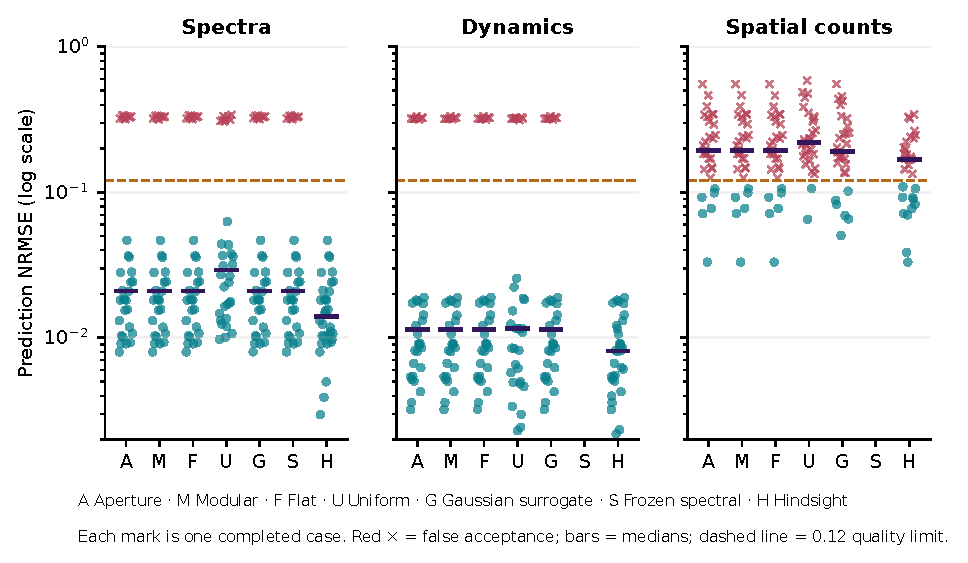
\includegraphics[width=\linewidth]{figures/all-case-errors.pdf}
\caption{\textbf{Measured error for every completed case.} The dashed line is the predeclared NRMSE limit of 0.12; crosses mark scientifically wrong estimates accepted by verification. Medians exclude abstentions because those missions have no estimate. Waiting has no points, and the restricted specialist supplies estimates only for spectra. The logarithmic axis displays heterogeneous errors without treating them as uncertainty intervals.}
\label{fig:errors}
\end{figure}

\subsection{Conventional substitutes and the privileged reference}

Uniform selection qualifies 50/96. Its four paired losses relative to Aperture, with no qualification gains, all occur in held-out imaging: 2/32 versus 6/32. This is a finite-suite benefit of the conventional information-selection rule over this fixed-spread strategy. It is not evidence for a distinctive architectural advantage.

The Gaussian surrogate matches qualification on every case, despite different selected-action lists in 28 cases. Exact count-likelihood fitting is therefore unnecessary for the observed qualification count. Its error tradeoff is less simple: the held-out 90th percentile worsens from 0.3497 to 0.4265. Equal coverage and lower recorded computation do not establish dominance in tail quality.

The hindsight specialist qualifies 75/96: all 64 known-family cases and 11/32 held-out cases. It adds 21 paired qualifications and loses none here, but retains 19 false acceptances. Known calibration and failed-action identities do not solve all low-count cases within the budget. This greedy reference has privileged information and no global optimality certificate.

One retained case, \code{h-d19003f77ccb}, reports an unsuccessful optimizer status for Aperture and flat. Both return NRMSE 0.345529, fail scientific quality and pass residual verification. Modular reports optimizer success with almost identical quality. The warning is preserved; neither case removal nor post-reveal solver repair is used to improve confirmation. Solver convergence and scientific correctness are separate questions.

\subsection{Observed costs and the costs still unknown}

Table~\ref{tab:compute} separates computation from the resource units in Table~\ref{tab:primary-results}. Aperture constructs 4,800 rows, evaluates 28,800 expression nodes and scores 102,240 candidate rows across the suite. It records eight recovery events and 53 waiting ticks. Sunk measurements removed during quarantine remain charged. Uniform avoids information scoring, while the Gaussian surrogate avoids Poisson objective calls.

\begin{table}[htbp]
\centering\small
\begin{tabularx}{\linewidth}{@{}Xrrrr@{}}
\toprule
\textbf{Method} & \textbf{Wall (s)} & \textbf{CPU (s)} & \textbf{Fits} & \shortstack{\textbf{Objective}\\\textbf{calls}}\\
\midrule
\ap{} & 2.002 & 2.001 & 2,066 & 12,677\\
Modular control & 2.001 & 2.000 & 2,066 & 12,622\\
Flat replacement & 2.138 & 2.138 & 2,066 & 12,677\\
Uniform selection & 2.016 & 2.015 & 2,072 & 14,157\\
Gaussian surrogate & 1.178 & 1.178 & 2,066 & 0\\
Frozen spectral & 0.213 & 0.213 & 672 & 0\\
Wait & 0.000513 & 0.000385 & 0 & 0\\
Hindsight specialist & 2.005 & 2.004 & 2,064 & 12,099\\
\bottomrule
\end{tabularx}
\caption{\textbf{Observed computational work across 96 missions.} Times sum the measured solve calls, including their construction and checks. Methods execute in fixed order in one recorded environment; these are descriptive timings, not randomized timing estimates. Objective calls count the nonlinear count objective; zero does not mean zero computational work.}
\label{tab:compute}
\end{table}

\begin{figure}[htbp]
\centering
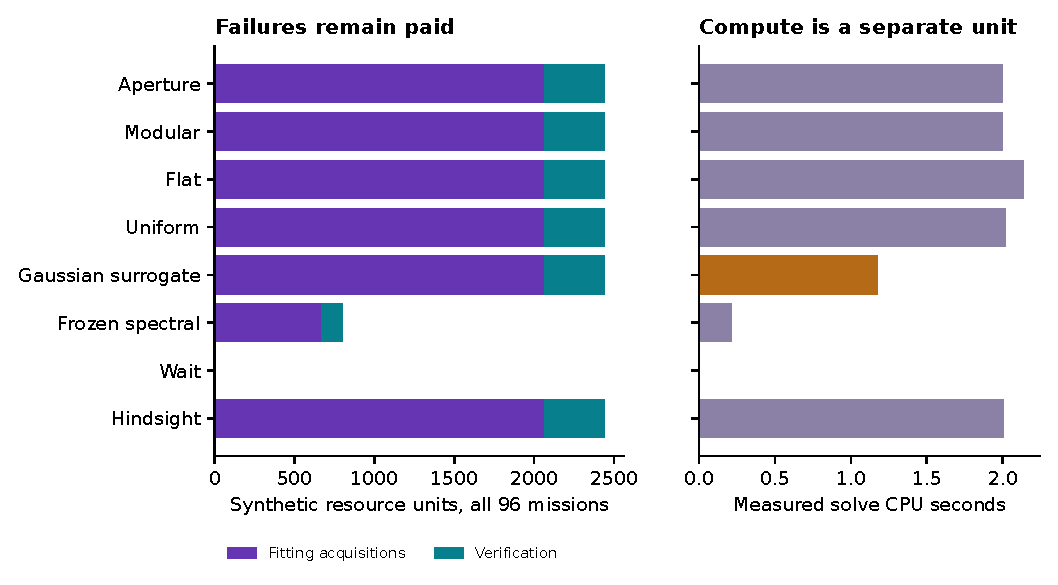
\includegraphics[width=\linewidth]{figures/full-observed-costs.pdf}
\caption{\textbf{Measured resource ledger.} Fitting and verification units include failed work; CPU seconds are shown separately. Lower costs for the restricted specialist reflect refusal of two families, and waiting produces no scientific output. The chart displays all observed costs in these dimensions, not a complete economic cost.}
\label{fig:costs}
\end{figure}

The surrogate's recorded 1.178 seconds versus Aperture's 2.002 seconds is useful implementation evidence, with no claim of a portable speed ratio. Attributable engineering, human review, provider computation, physical instruments, energy, prices and future maintenance remain unknown. Operational budget matching does not establish equal total human effort. A positive additional architecture cost cannot be recovered through repeated numerical and acquisition ties without another measured benefit.

\subsection{Demand shifts reveal the price of preserving options}

The replay contains 288 conditions, including 96 matched Aperture/modular pairs. Every pair agrees in qualified outputs, used units, completed attempts and false acceptances. These are repeated sensitivity calculations on selected cases, not additional independent demand observations.

The first replay attempt stopped before execution because steward stress labels did not match the frozen lookup names. A disclosed post-reveal metadata adapter maps normal to nominal, correlated calibration failure to calibration failure, and unavailable action group to capacity loss. Raw labels, the failed attempt and both file hashes are retained. Scientific records and frozen policy are unchanged. This reconciliation does not assert equal stress severity across families.

At capacity 90 and an assumed three-unit family-switch tariff, eager execution yields three qualified stable-family outputs for 84 units, three shifted-family outputs for 90 units, and zero qualified shared-failure outputs for 90 units. The last schedule produces three false acceptances. Stopping after failed verification cannot help when all three wrong outputs pass that check. At a twelve-unit tariff the shifted schedule fits only two qualified outputs into capacity, while stable demand still yields three.

\begin{figure}[htbp]
\centering
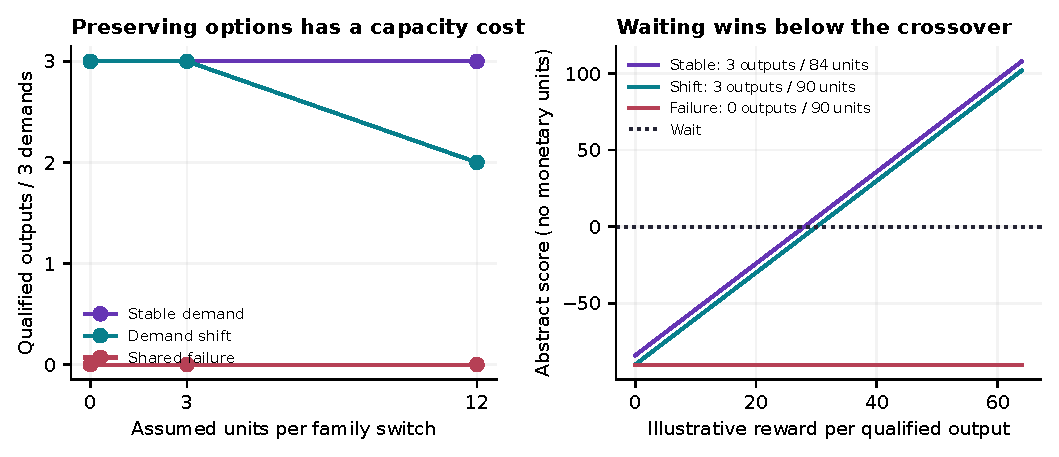
\includegraphics[width=\linewidth]{figures/option-cost-crossovers.pdf}
\caption{\textbf{Conditional replay and illustrative valuation.} At capacity 90, the left panel varies an assumed switch tariff. The right panel uses a three-unit tariff and the toy score $RQ-U$: reward $R$ per qualified output, observed resource units $U$. Rewards are illustrative units, not prices, receipts or willingness to pay. These curves describe the chosen schedules only.}
\label{fig:crossovers}
\end{figure}

For the illustrative score $RQ-U$, stable and shifted execution cross waiting's zero score at $R=28$ and $R=30$, respectively. Below those thresholds waiting does better under this chosen accounting; the shared-failure schedule remains at $-90$ for any nonnegative reward because it produces no qualified output. These are transparent conditional crossovers, not option prices or market forecasts. They omit unmeasured costs and the value of opportunities forgone by waiting. Flexibility expands an executable task set, but cannot rescue false evidence, eliminate switching costs or establish positive economic alpha by itself.


\section{Project foundations and their actual integration}\label{sec:foundations}

The experiment uses the complete current \emph{Transformational Intelligence} manuscript as a methodological foundation \citep{boucher2026ti}. Its formulation separates representations, world assumptions, information channels, policy language and intermediate targets from the user's purpose and external permissions. It also reports a conventional unrestricted planner matching its illustrative active policy. We follow that discipline: changed attainable actions and superiority over an equally enabled builder are separate questions.

The requested connected journey is \textbf{Identify $\to$ Out-Learn $\to$ Out-Think $\to$ Out-Design $\to$ Out-Strategise $\to$ Out-Execute $\to$ Out-Evolve}. Identify fixes the authorized scientific question and budgets. Out-Learn reads the primary literature and public reference data. Out-Think uses the pilot to reject known-model fitting as the bottleneck. Out-Design constructs the measurement program. Out-Strategise freezes its comparison and stopping conditions. Out-Execute produces the bounded measurements and checks. Out-Evolve preserves counterexamples and identifies a separately authorized successor experiment. These labels describe connected responsibilities, not seven required transactions.

\begin{table}[htbp]
\centering\small
\begin{tabularx}{\linewidth}{@{}p{.20\linewidth}p{.21\linewidth}X@{}}
\toprule
\textbf{Repository} & \textbf{Inspected commit} & \textbf{Source-backed role and current scope}\\
\midrule
Alpha & \texttt{197147ffd22c} & Real native dispatcher and state/journal objects; seven-stage local integration and source audit.\\
Jobs Manager & \texttt{c5958eae8724} & Existing inspector can create an unfunded USDC6 proposal for supported inputs; new scientific family not demonstrated as admitted.\\
Jobs v0 & \texttt{9983478d42c3} & Separate AGIALPHA18 proposal route with source/evaluation bindings; no settlement in this study.\\
Fleet Linux & \texttt{45759fb096fa} & Current inspected mapping supports a fixed public-data row-total family; numerical missions require a new reviewed mapping and authority.\\
\bottomrule
\end{tabularx}
\caption{Pinned source audit \citep{alpha2026source,manager2026source,jobs2026source,fleet2026source}. Full commit identifiers, immutable source URLs, licenses and 74 file identities appear in the evidence package. A conceptual mapping is not reported as a working four-repository integration.}
\end{table}

The thin integration imports the unchanged published Alpha \code{JobDispatcher} and \code{SuccessorStore}. Its seven source job families are constitution, evidence, challenge, formation, admission, verification and renewal; the mapping to the user-facing pipeline is explicit. It executes reviewed bounded pure callbacks, not arbitrary generated host code. The final trace audits already completed evidence and executes one known development case. It does not claim that the dispatcher caused or planned the earlier confirmation sample.

The customer-facing World, Policy, Proof and Authority objects are inspectable JSON. World contains the current mission and observations; Policy identifies the frozen method and plan; Proof contains source-bound results and limitations; Authority states the existing local scope and expiry. The artifact's restoration tests are executed. Native Alpha portable export/restore remains unexecuted because its lazy settlement import closure reached a missing dependency after two retained failed attempts. Those native properties are source observations, not new test results. Local EVM installation also stopped with storage exhaustion before contract tests; the installation failure and exit status are preserved. No live-chain substitute was used.

\subsection{Five contracts, five carefully bounded roles}

\textbf{AscensionAccess} checks current ENS ownership and expiring admission for the business, agent and validator roots. Eligibility is not competence or permission for new work. \textbf{NovaSeed} commits capsule, plan, evidence and lineage data; its inspected source has no setter to expand an existing committed plan. A material new opportunity therefore needs a fresh seed and separate evidence, budget and authority.

\textbf{AscensionRiskOracle} uses staked, expiring, owner-bound reviews and reserves review capacity. Distinct addresses do not establish organizational independence. \textbf{AscensionJobMarket} implements bounded auctions, worker bonds, artifact-bound voting and payout/refund/timeout rules. Its economic effects follow the implemented protocol; votes are not a proof of scientific correctness.

\textbf{AscensionMark} implements None $\to$ Funding $\to$ Bloomed $\to$ Closed. Funding $\to$ Bloomed requires the source-specified reserve, current green review, ownership and ENS conditions. Later jobs remain inside the immutable Merkle plan, treasury and horizon. A bloom is a lifecycle transition, not wealth, realized profit or ownership of later opportunities.

Applicable AGIALPHA18 utility includes stakes, job bounties, campaign reserves, payouts and burns. Manager's USDC6 route remains separate. These source mechanics neither imply token appreciation nor make a token necessary for this local scientific laboratory. The source audit is not a contract-execution demonstration; local EVM tests were not run.

\section{Limitations and the next falsifiable study}

\textbf{Finite construction language.} The held-out family is unseen to the builder before freeze but lies inside a predeclared grammar. The system does not invent its basis, likelihood or solver from raw science. New physics, incompatible interfaces and higher-dimensional models may require replacement. Three scientific missions sharing an inverse-problem core cannot support universal flexibility.

\textbf{Conditional scientific verification.} The residual check is model-conditional and is not a calibrated confidence guarantee. Shared calibration error can fool it. Synthetic validation truth makes that failure visible; a physical experiment would need a genuinely independent reference, calibrated instrument or intervention. The study's purpose bridge uses that truth only in evaluation, not to select ordinary-policy actions.

\textbf{Comparative and economic limits.} A shared conventional implementation is a strong control against invented construction privilege, but does not measure real expert productivity, maintenance burden, operator comprehension or total human engineering cost. Timings are single-environment observations, not a general performance benchmark. Unknown costs prevent a net-value claim. The hindsight reference has extra information and no global optimality certificate.

\textbf{Synthetic demand and correlated failures.} The sequences, capacities and switch tariffs are explicitly chosen scenarios. Their averages are not expected market returns. Sensitivity over observed strata cannot bound behavior in an unrepresented future. Repeated replay conditions are not independent samples. A common component can fail across several apparently different tasks.

\textbf{Integration and custody.} The complete publication is reviewable and reproducible, but publication, qualified software release, live Pages acceptance, Fleet admission and contract settlement are distinct states. The existing publication coordinator retains shared-index, merge and deployment ownership. Local tests cannot waive a held action or transfer review authority.

The next useful test is specific: recruit independent builders, prospectively log engineering and review effort, introduce task families requiring primitives outside the current grammar, and compare repeated delivery at a common independently validated quality level. A physical or operational pilot should then measure demand, actual usage, willingness to pay, maintenance, failures and realized receipts. Those observations could establish a construction-cost crossover that this bounded study cannot.

\section{Reproduce, inspect and use the artifact}

The authoritative PDF is inside the complete ZIP with LaTeX, bibliography, vector figures, source, the original sealed generator, reveal chronology, frozen hashes, all results, source audits, environment information, tests and an evidence index. The top-level README supplies exact commands. A clean extracted directory is used for the numerical rerun and manuscript rebuild. Numerical and event records are compared after excluding measured timing fields; performance timings are not expected to reproduce byte-for-byte.

Run the local demonstration to reveal a different demand, authorize bounded synthetic work, reconstruct the measurement program, inspect costs and scientific quality, and export or restore the four objects. An imported snapshot cannot issue its own current authority. The demonstration requires no wallet, private data, paid account or privileged service. Any static evidence-replay mode is labeled separately from a fresh Python execution.

The practical outcome is an instrument a reader can inspect and change within a finite contract. Its value is not that it eliminates the need to predict or that it beats every conventional method. It makes one concrete kind of adaptation executable, its price visible, and its failures available for the next design decision.


\appendix
\section{Contracts, costs and evidence custody}

\begin{table}[htbp]
\centering\small
\begin{tabularx}{\linewidth}{@{}p{.23\linewidth}XX@{}}
\toprule
\textbf{Component} & \textbf{Before demand is revealed} & \textbf{After reveal; boundary}\\
\midrule
Response language & Installed finite AST, parser and arity/depth checks & Compose supported expressions; unknown operation refuses\\
Measurement operator & Weighted-aggregation rule and finite point budget & Construct mission-specific rows; over-budget input refuses\\
Inference & Gaussian joint MAP and nonnegative Poisson MAP & Choose the declared installed likelihood; new law needs development\\
Action policy & Greedy design, repetition limits, ledger and health filter & Use current evidence; quarantine only within authorized scope\\
Verification & Four reserved actions and fixed residual threshold & Record acceptance and independent evaluation disagreement\\
Evidence objects & World, Policy, Proof, Authority contracts & Export/inspect; restore only under separately current permission\\
External work & No wallet or external settlement authority & New mission requires fresh seed and bounded grant\\
\bottomrule
\end{tabularx}
\caption{What is constructed, reconfigured or replaced. The installed representation makes specified transformations possible; it does not grant arbitrary new actions.}
\end{table}

Mission inputs are public JSON with finite numeric values, explicit likelihood, basis expressions, weighted candidate points, action-group labels, costs, fitting budget, verification count and quality threshold. Outputs include the constructed-plan identity, inferred coefficients, selected actions, observations, solver status, every ledger event, quality and verification results, and source-bound export objects. The hidden evaluator's scientific truth is stored separately. Construction rejects excessive dimensions, recursion, invalid values and unsupported likelihoods; execution refuses missing, expired or incompatible authority. An invalid observation spends its declared cost and triggers recorded recovery. A failed result is not repaired with unrecorded work.

The cost ledger is a vector rather than a single price. Construction counts rows, basis-node work and measured setup time. Execution counts all acquisition calls and units, likelihood objectives, solver invocations and candidate scores. Verification counts reserved measurements and their costs. Recovery preserves sunk observations and refits. Waiting retains ticks; campaign switching uses declared synthetic tariffs. Wall and CPU scopes are separately stated. Long-lived maintenance, energy, instrument wear, commercial overhead, human engineering, model-provider compute and monetary conversion are unknown. There is no positive realized-receipts claim.

\section{Reproducibility and checks}

The complete package's evidence index connects every central claim to its source. The commands below are run from the extracted package root in a Python environment with the published dependencies. The reproduction wrapper requires a new output directory and verifies the frozen source before execution. The manuscript build uses ordinary \LaTeX{} tools and supplied vector figures.

\begin{minipage}{\linewidth}
\begin{verbatim}
python reproduce.py --output evidence/reproduced
bash build_paper.sh
python demo/server.py
\end{verbatim}
\end{minipage}

The bounded numerical environment uses Python, NumPy 2.3.5 and SciPy 1.17.0. BLAS and OpenMP threads are set to one. Matplotlib 3.10.8 produces the reporting figures. Exact versions and platform details are machine-readable in the evidence. Reproduction compares scientific and event fields after excluding measured timing fields; a fresh machine or numerical-library change may require a declared tolerance-based follow-up, not an unreported change to the original exact comparison. Native integration dependencies are separate from the minimal scientific program.

Twenty-two independent pre-freeze tests cover numerical inference, data validation, timing/authority boundaries, flat-plan tampering, observation-prefix information flow, sunk recovery costs and late health events. The frozen checker verifies all 768 primary records against event counts, quality, budgets and authority. A separate held-out audit performs 29,136 checks across 256 method records, independently regenerating 5,040 noise observations, 180 non-abstaining quality values and 720 verification residuals. It also checks 40 quarantine events at their actual reveal tick and verifies all 39 frozen file identities. Its maximum independent quality discrepancy is $5.55\times10^{-17}$ and maximum residual discrepancy $1.64\times10^{-14}$. These are deterministic consistency checks, not 29,136 independent scientific experiments.

The local demonstration has 12 focused tests, including real loopback HTTP requests and a bounded numerical run. They test explicit consent, a spent one-run grant, exact restoration, edited and rehashed authority, forged proof, real-time expiry, server restart, incompatible missions, duplicate/nonfinite JSON, and static replay bindings. A cloud browser could not connect to the loopback service in the separate execution environment; browser visual validation is marked unexecuted. The publication's PDF pages are rendered and inspected separately.

The final native dispatcher trace records seven callbacks and 46 verified journal events. Three source-native refusal cases cover expired authority, incompatible environment and immutable changed terms. The artifact's own six restore checks execute, while source-native portable restoration and EVM contract execution remain \texttt{NOT\_RUN}, with their dependency/storage failures preserved. The integration's one known-case solve reaches NRMSE 0.01325 with 24 fitting units and four verification units. Its 420 prepared potential observations are computational preparation, not claimed instrument measurements.

\section{Registered identities and repository provenance}

The protocol freeze was created at \texttt{2026-10-24T02:59:29.333081+00:00}. The sealed generator existed before that time; its cases were materialized only after the verified frozen checkpoint and public coordination note. The retained chronology identifies each step and its actual scope. A later replay-label adapter, reporting scripts, demonstration and manuscript are explicitly outside the scientific freeze.

\begin{description}[style=nextline,leftmargin=0pt,labelwidth=0pt,labelsep=0pt,font=\normalfont\bfseries]
\item[Scientific source and protocol freeze (39 files)]
\path{147678382894e349fd53236e68447cb640110e25aa401ae5c7f19d0be6528076}
\item[Preconfirmation complete checkpoint ZIP]
\path{9abe05352d59e7425a0a4a5d5dff721c6d4ce6ac1647982b845b26817c854b36}
\item[Original sealed generator archive]
\path{6bfc5076c2ea4b8f40acb01dac862e87975facdf71591a0f9768fa78cc6a13a4}
\item[Recorded 768 primary outcomes]
\path{7544bb57d785a9f1b2fdb08ec52bc817a54b81601141113641ca10ab506e8e5c}
\item[Timing-independent scientific record digest]
\path{a2212a7c5b078892c87308e4c03fd111e3161a1cff5b0b141c27bdd00b421ee7}
\end{description}

All repository identities below are immutable audited commits, not claims that the current default branch is unchanged:

\begin{description}[style=nextline,leftmargin=0pt,labelwidth=0pt,labelsep=0pt,font=\normalfont\bfseries]
\item[AGI-Alpha-Agent-v0]
\url{https://github.com/MontrealAI/AGI-Alpha-Agent-v0}\\
\path{197147ffd22c5ae13113162afffaf3ce9c10aa2e}
\item[AGIJobsv0]
\url{https://github.com/MontrealAI/AGIJobsv0}\\
\path{9983478d42c32fe399f28dd9b0e0173f904b8a11}
\item[AGIJobManager]
\url{https://github.com/MontrealAI/AGIJobManager}\\
\path{c5958eae872458c2f3cac48fea0b4bbfadc6ac6c}
\item[AGI-Fleet-Linux]
\url{https://github.com/MontrealAI/AGI-Fleet-Linux}\\
\path{45759fb096faf8988f58ae5ea71248d0f35a97c7}
\end{description}

The source audit preserves licenses and file identities. Third-party source retains its original license and attribution. NIST raw data are retrieved separately under their source instructions; synthetic scenario data and derived permitted outputs are packaged. The final manifest binds all delivered files and the authoritative PDF inside the ZIP. Reopening a saved ZIP and verifying its manifest establishes byte custody, not the truth of a scientific model.

\section{Pipeline and public release boundary}

\begin{table}[H]
\centering\small
\begin{tabularx}{\linewidth}{@{}p{.18\linewidth}XX@{}}
\toprule
\textbf{TI stage} & \textbf{Executed evidence} & \textbf{Explicit limitation}\\
\midrule
Identify & Mission contract, purpose threshold and bounded authority & Synthetic scientific objective, no market validation\\
Out-Learn & Primary literature, four repository audits, NIST pilot & No exhaustive search or physical instrument survey\\
Out-Think & Cheap conventional fitting falsifies an initial bottleneck & No measured human reasoning benchmark\\
Out-Design & Finite representation and actual operator construction & Primitives supplied before reveal\\
Out-Strategise & Frozen comparator, stopping and stress protocol & No inferred probability of future demand\\
Out-Execute & 768 records, 288 replays, audit and local integration & Native EVM and portable restore not executed\\
Out-Evolve & Failure record, export/restore and next-study specification & New work needs fresh evidence and authority\\
\bottomrule
\end{tabularx}
\caption{The complete connected TI pipeline applied to this experiment. SUCCESSOR $\Omega$ supplies a thin source-native dispatch and audit integration; it is not introduced as another standalone framework.}
\end{table}

The authorized public destination is the Alpha repository and its existing GitHub Pages site. The coordination issue is \url{https://github.com/MontrealAI/AGI-Alpha-Agent-v0/issues/4850}. The current publication owner retains shared catalog, merge and Pages responsibilities. This research can be reviewed in a focused additive author namespace; locally completed files do not establish acceptance or deployment. The package handoff records the exact reviewed identities and publication state without treating a source PR as an already live Pages release.

\begingroup
\raggedright
\small
\setlength{\bibsep}{.4em}
\begin{thebibliography}{21}
\providecommand{\natexlab}[1]{#1}
\providecommand{\url}[1]{\texttt{#1}}
\expandafter\ifx\csname urlstyle\endcsname\relax
  \providecommand{\doi}[1]{doi: #1}\else
  \providecommand{\doi}{doi: \begingroup \urlstyle{rm}\Url}\fi

\bibitem[Baldwin and Clark(2002)]{baldwin2002option}
Carliss~Y. Baldwin and Kim~B. Clark.
\newblock The option value of modularity in design: An example from design
  rules, volume 1: The power of modularity.
\newblock Technical Report 02-078, Harvard Business School, 2002.
\newblock URL \url{https://scholarsarchive.byu.edu/facpub/8944/}.

\bibitem[Ben-Tal et~al.(2004)Ben-Tal, Goryashko, Guslitzer, and
  Nemirovski]{bental2004adjustable}
Aharon Ben-Tal, Alexander Goryashko, Elana Guslitzer, and Arkadi Nemirovski.
\newblock Adjustable robust solutions of uncertain linear programs.
\newblock \emph{Mathematical Programming}, 99:\penalty0 351--376, 2004.
\newblock \doi{10.1007/s10107-003-0454-y}.
\newblock URL \url{https://www2.isye.gatech.edu/~nemirovs/MP_Elana_2004.pdf}.

\bibitem[Bertsimas and Sim(2004)]{bertsimas2004price}
Dimitris Bertsimas and Melvyn Sim.
\newblock The price of robustness.
\newblock \emph{Operations Research}, 52\penalty0 (1):\penalty0 35--53, 2004.
\newblock \doi{10.1287/opre.1030.0065}.
\newblock URL
  \url{https://www.mit.edu/~dbertsim/papers/melvyn/The-Price-Of-Robustness-OR52.pdf}.

\bibitem[Boucher(2026)]{boucher2026ti}
Vincent Boucher.
\newblock Transformational intelligence: Learning to change the game.
\newblock MONTREAL.AI research manuscript, 24 pages, 2026.
\newblock URL
  \url{https://github.com/MontrealAI/AGI-Alpha-Agent-v0/blob/197147ffd22c5ae13113162afffaf3ce9c10aa2e/docs/Transformational_Intelligence.pdf}.
\newblock Pinned source, Git blob 1f95db3b087d8dd0712012d34ba700d7dd2e1382;
  source audit in companion.

\bibitem[Brunton et~al.(2016)Brunton, Proctor, and Kutz]{brunton2016sindy}
Steven~L. Brunton, Joshua~L. Proctor, and J.~Nathan Kutz.
\newblock Discovering governing equations from data by sparse identification of
  nonlinear dynamical systems.
\newblock \emph{Proceedings of the National Academy of Sciences}, 113\penalty0
  (15):\penalty0 3932--3937, 2016.
\newblock \doi{10.1073/pnas.1517384113}.
\newblock URL \url{https://arxiv.org/abs/1509.03580}.

\bibitem[Foster et~al.(2019)Foster, Jankowiak, Bingham, Horsfall, Teh,
  Rainforth, and Goodman]{foster2019design}
Adam Foster, Martin Jankowiak, Eli Bingham, Paul Horsfall, Yee~Whye Teh, Tom
  Rainforth, and Noah Goodman.
\newblock Variational {Bayesian} optimal experimental design.
\newblock In \emph{Advances in Neural Information Processing Systems},
  volume~32, 2019.
\newblock URL
  \url{https://papers.nips.cc/paper_files/paper/2019/hash/d55cbf210f175f4a37916eafe6c04f0d-Abstract.html}.

\bibitem[Golub and Pereyra(1973)]{golub1973separable}
Gene~H. Golub and Victor Pereyra.
\newblock The differentiation of pseudo-inverses and nonlinear least squares
  problems whose variables separate.
\newblock \emph{SIAM Journal on Numerical Analysis}, 10\penalty0 (2):\penalty0
  413--432, 1973.
\newblock \doi{10.1137/0710036}.
\newblock URL \url{https://epubs.siam.org/doi/10.1137/0710036}.

\bibitem[Haasnoot et~al.(2013)Haasnoot, Kwakkel, Walker, and ter
  Maat]{haasnoot2013pathways}
Marjolijn Haasnoot, Jan~H. Kwakkel, Warren~E. Walker, and Judith ter Maat.
\newblock Dynamic adaptive policy pathways: A method for crafting robust
  decisions for a deeply uncertain world.
\newblock \emph{Global Environmental Change}, 23\penalty0 (2):\penalty0
  485--498, 2013.
\newblock \doi{10.1016/j.gloenvcha.2012.12.006}.
\newblock URL
  \url{https://ris.utwente.nl/ws/files/247793059/Haasnoot2013dynamic.pdf}.

\bibitem[Joshi and Boyd(2009)]{joshi2009sensors}
Siddharth Joshi and Stephen Boyd.
\newblock Sensor selection via convex optimization.
\newblock \emph{IEEE Transactions on Signal Processing}, 57\penalty0
  (2):\penalty0 451--462, 2009.
\newblock \doi{10.1109/TSP.2008.2007095}.
\newblock URL
  \url{https://web.stanford.edu/~boyd/papers/sensor_selection.html}.

\bibitem[Koren et~al.(1999)Koren, Heisel, Jovane, Moriwaki, Pritschow, Ulsoy,
  and Van~Brussel]{koren1999reconfigurable}
Y.~Koren, U.~Heisel, F.~Jovane, T.~Moriwaki, G.~Pritschow, G.~Ulsoy, and
  H.~Van~Brussel.
\newblock Reconfigurable manufacturing systems.
\newblock \emph{CIRP Annals}, 48\penalty0 (2):\penalty0 527--540, 1999.
\newblock \doi{10.1016/S0007-8506(07)63232-6}.
\newblock URL
  \url{https://public.websites.umich.edu/~ykoren/uploads/Reconfigurable_manufacturing_systems_1999_keynote_paper.pdf}.

\bibitem[Lempert et~al.(2003)Lempert, Popper, and Bankes]{lempert2003shaping}
Robert~J. Lempert, Steven~W. Popper, and Steven~C. Bankes.
\newblock Shaping the next one hundred years: New methods for quantitative,
  long-term policy analysis.
\newblock Technical Report MR-1626-RPC, RAND Corporation, 2003.
\newblock URL \url{https://www.rand.org/pubs/monograph_reports/MR1626.html}.

\bibitem[Ma et~al.(2021)Ma, Gowda, Anantharaman, Laughman, Shah, and
  Rackauckas]{ma2021modelingtoolkit}
Yingbo Ma, Shashi Gowda, Ranjan Anantharaman, Chris Laughman, Viral Shah, and
  Chris Rackauckas.
\newblock {ModelingToolkit}: A composable graph transformation system for
  equation-based modeling, 2021.
\newblock URL \url{https://arxiv.org/abs/2103.05244v3}.
\newblock Version 3 revised February 9, 2022.

\bibitem[McDonald and Siegel(1986)]{mcdonald1986waiting}
Robert McDonald and Daniel Siegel.
\newblock The value of waiting to invest.
\newblock \emph{The Quarterly Journal of Economics}, 101\penalty0 (4):\penalty0
  707--727, 1986.
\newblock \doi{10.2307/1884175}.
\newblock URL
  \url{https://academic.oup.com/qje/article-abstract/101/4/707/1840173}.
\newblock Earlier working-paper version: NBER Working Paper 1019, 1982,
  https://www.nber.org/papers/w1019.

\bibitem[{MONTREAL.AI}(2026{\natexlab{a}})]{alpha2026source}
{MONTREAL.AI}.
\newblock {AGI-Alpha-Agent-v0}: audited source snapshot, 2026{\natexlab{a}}.
\newblock URL
  \url{https://github.com/MontrealAI/AGI-Alpha-Agent-v0/tree/197147ffd22c5ae13113162afffaf3ce9c10aa2e}.
\newblock Commit 197147ffd22c5ae13113162afffaf3ce9c10aa2e; Apache-2.0.

\bibitem[{MONTREAL.AI}(2026{\natexlab{b}})]{fleet2026source}
{MONTREAL.AI}.
\newblock {AGI-Fleet-Linux}: audited source snapshot, 2026{\natexlab{b}}.
\newblock URL
  \url{https://github.com/MontrealAI/AGI-Fleet-Linux/tree/45759fb096faf8988f58ae5ea71248d0f35a97c7}.
\newblock Commit 45759fb096faf8988f58ae5ea71248d0f35a97c7; MIT.

\bibitem[{MONTREAL.AI}(2026{\natexlab{c}})]{jobs2026source}
{MONTREAL.AI}.
\newblock {AGIJobsv0}: audited source snapshot, 2026{\natexlab{c}}.
\newblock URL
  \url{https://github.com/MontrealAI/AGIJobsv0/tree/9983478d42c32fe399f28dd9b0e0173f904b8a11}.
\newblock Commit 9983478d42c32fe399f28dd9b0e0173f904b8a11; MIT.

\bibitem[{MONTREAL.AI}(2026{\natexlab{d}})]{manager2026source}
{MONTREAL.AI}.
\newblock {AGIJobManager}: audited source snapshot, 2026{\natexlab{d}}.
\newblock URL
  \url{https://github.com/MontrealAI/AGIJobManager/tree/c5958eae872458c2f3cac48fea0b4bbfadc6ac6c}.
\newblock Commit c5958eae872458c2f3cac48fea0b4bbfadc6ac6c; MIT.

\bibitem[{National Institute of Standards and Technology}()]{nistlicense}
{National Institute of Standards and Technology}.
\newblock Copyright, fair use, and licensing statements for {SRD}, data,
  software, and technical series publications.
\newblock URL \url{https://www.nist.gov/open/license}.
\newblock Accessed for the Writer 11 study; distinguishes SRD products from
  other NIST data.

\bibitem[Parnas(1972)]{parnas1972modules}
David~L. Parnas.
\newblock On the criteria to be used in decomposing systems into modules.
\newblock \emph{Communications of the ACM}, 15\penalty0 (12):\penalty0
  1053--1058, 1972.
\newblock \doi{10.1145/361598.361623}.
\newblock URL \url{https://doi.org/10.1145/361598.361623}.

\bibitem[Rust(1996)]{nist1996gauss1}
B.~Rust.
\newblock {Gauss1}: {NIST} statistical reference datasets.
\newblock National Institute of Standards and Technology, 1996.
\newblock URL \url{https://www.itl.nist.gov/div898/strd/nls/data/gauss1.shtml}.
\newblock Public generated nonlinear-regression reference dataset; 250
  observations; collection SRD 140, DOI 10.18434/T43G6C.

\bibitem[Solar-Lezama(2008)]{solarlezama2008sketching}
Armando Solar-Lezama.
\newblock \emph{Program Synthesis by Sketching}.
\newblock PhD thesis, University of California, Berkeley, 2008.
\newblock URL
  \url{https://www2.eecs.berkeley.edu/Pubs/TechRpts/2008/EECS-2008-176.html}.
\newblock Technical Report UCB/EECS-2008-176.

\end{thebibliography}

\endgroup
\end{document}
